\documentclass[]{book}
\usepackage{lmodern}
\usepackage{amssymb,amsmath}
\usepackage{ifxetex,ifluatex}
\usepackage{fixltx2e} % provides \textsubscript
\ifnum 0\ifxetex 1\fi\ifluatex 1\fi=0 % if pdftex
  \usepackage[T1]{fontenc}
  \usepackage[utf8]{inputenc}
\else % if luatex or xelatex
  \ifxetex
    \usepackage{mathspec}
  \else
    \usepackage{fontspec}
  \fi
  \defaultfontfeatures{Ligatures=TeX,Scale=MatchLowercase}
\fi
% use upquote if available, for straight quotes in verbatim environments
\IfFileExists{upquote.sty}{\usepackage{upquote}}{}
% use microtype if available
\IfFileExists{microtype.sty}{%
\usepackage{microtype}
\UseMicrotypeSet[protrusion]{basicmath} % disable protrusion for tt fonts
}{}
\usepackage[margin=1in]{geometry}
\usepackage{hyperref}
\hypersetup{unicode=true,
            pdftitle={GraphQL workshop for NodeJS developers},
            pdfauthor={Iván Corrales Solera ivan.corrales.solera@gmail.com},
            pdfborder={0 0 0},
            breaklinks=true}
\urlstyle{same}  % don't use monospace font for urls
\usepackage{natbib}
\bibliographystyle{apalike}
\usepackage{color}
\usepackage{fancyvrb}
\newcommand{\VerbBar}{|}
\newcommand{\VERB}{\Verb[commandchars=\\\{\}]}
\DefineVerbatimEnvironment{Highlighting}{Verbatim}{commandchars=\\\{\}}
% Add ',fontsize=\small' for more characters per line
\usepackage{framed}
\definecolor{shadecolor}{RGB}{248,248,248}
\newenvironment{Shaded}{\begin{snugshade}}{\end{snugshade}}
\newcommand{\KeywordTok}[1]{\textcolor[rgb]{0.13,0.29,0.53}{\textbf{#1}}}
\newcommand{\DataTypeTok}[1]{\textcolor[rgb]{0.13,0.29,0.53}{#1}}
\newcommand{\DecValTok}[1]{\textcolor[rgb]{0.00,0.00,0.81}{#1}}
\newcommand{\BaseNTok}[1]{\textcolor[rgb]{0.00,0.00,0.81}{#1}}
\newcommand{\FloatTok}[1]{\textcolor[rgb]{0.00,0.00,0.81}{#1}}
\newcommand{\ConstantTok}[1]{\textcolor[rgb]{0.00,0.00,0.00}{#1}}
\newcommand{\CharTok}[1]{\textcolor[rgb]{0.31,0.60,0.02}{#1}}
\newcommand{\SpecialCharTok}[1]{\textcolor[rgb]{0.00,0.00,0.00}{#1}}
\newcommand{\StringTok}[1]{\textcolor[rgb]{0.31,0.60,0.02}{#1}}
\newcommand{\VerbatimStringTok}[1]{\textcolor[rgb]{0.31,0.60,0.02}{#1}}
\newcommand{\SpecialStringTok}[1]{\textcolor[rgb]{0.31,0.60,0.02}{#1}}
\newcommand{\ImportTok}[1]{#1}
\newcommand{\CommentTok}[1]{\textcolor[rgb]{0.56,0.35,0.01}{\textit{#1}}}
\newcommand{\DocumentationTok}[1]{\textcolor[rgb]{0.56,0.35,0.01}{\textbf{\textit{#1}}}}
\newcommand{\AnnotationTok}[1]{\textcolor[rgb]{0.56,0.35,0.01}{\textbf{\textit{#1}}}}
\newcommand{\CommentVarTok}[1]{\textcolor[rgb]{0.56,0.35,0.01}{\textbf{\textit{#1}}}}
\newcommand{\OtherTok}[1]{\textcolor[rgb]{0.56,0.35,0.01}{#1}}
\newcommand{\FunctionTok}[1]{\textcolor[rgb]{0.00,0.00,0.00}{#1}}
\newcommand{\VariableTok}[1]{\textcolor[rgb]{0.00,0.00,0.00}{#1}}
\newcommand{\ControlFlowTok}[1]{\textcolor[rgb]{0.13,0.29,0.53}{\textbf{#1}}}
\newcommand{\OperatorTok}[1]{\textcolor[rgb]{0.81,0.36,0.00}{\textbf{#1}}}
\newcommand{\BuiltInTok}[1]{#1}
\newcommand{\ExtensionTok}[1]{#1}
\newcommand{\PreprocessorTok}[1]{\textcolor[rgb]{0.56,0.35,0.01}{\textit{#1}}}
\newcommand{\AttributeTok}[1]{\textcolor[rgb]{0.77,0.63,0.00}{#1}}
\newcommand{\RegionMarkerTok}[1]{#1}
\newcommand{\InformationTok}[1]{\textcolor[rgb]{0.56,0.35,0.01}{\textbf{\textit{#1}}}}
\newcommand{\WarningTok}[1]{\textcolor[rgb]{0.56,0.35,0.01}{\textbf{\textit{#1}}}}
\newcommand{\AlertTok}[1]{\textcolor[rgb]{0.94,0.16,0.16}{#1}}
\newcommand{\ErrorTok}[1]{\textcolor[rgb]{0.64,0.00,0.00}{\textbf{#1}}}
\newcommand{\NormalTok}[1]{#1}
\usepackage{longtable,booktabs}
\usepackage{graphicx,grffile}
\makeatletter
\def\maxwidth{\ifdim\Gin@nat@width>\linewidth\linewidth\else\Gin@nat@width\fi}
\def\maxheight{\ifdim\Gin@nat@height>\textheight\textheight\else\Gin@nat@height\fi}
\makeatother
% Scale images if necessary, so that they will not overflow the page
% margins by default, and it is still possible to overwrite the defaults
% using explicit options in \includegraphics[width, height, ...]{}
\setkeys{Gin}{width=\maxwidth,height=\maxheight,keepaspectratio}
\IfFileExists{parskip.sty}{%
\usepackage{parskip}
}{% else
\setlength{\parindent}{0pt}
\setlength{\parskip}{6pt plus 2pt minus 1pt}
}
\setlength{\emergencystretch}{3em}  % prevent overfull lines
\providecommand{\tightlist}{%
  \setlength{\itemsep}{0pt}\setlength{\parskip}{0pt}}
\setcounter{secnumdepth}{5}
% Redefines (sub)paragraphs to behave more like sections
\ifx\paragraph\undefined\else
\let\oldparagraph\paragraph
\renewcommand{\paragraph}[1]{\oldparagraph{#1}\mbox{}}
\fi
\ifx\subparagraph\undefined\else
\let\oldsubparagraph\subparagraph
\renewcommand{\subparagraph}[1]{\oldsubparagraph{#1}\mbox{}}
\fi

%%% Use protect on footnotes to avoid problems with footnotes in titles
\let\rmarkdownfootnote\footnote%
\def\footnote{\protect\rmarkdownfootnote}

%%% Change title format to be more compact
\usepackage{titling}

% Create subtitle command for use in maketitle
\newcommand{\subtitle}[1]{
  \posttitle{
    \begin{center}\large#1\end{center}
    }
}

\setlength{\droptitle}{-2em}

  \title{GraphQL workshop for NodeJS developers}
    \pretitle{\vspace{\droptitle}\centering\huge}
  \posttitle{\par}
    \author{Iván Corrales Solera
\href{mailto:ivan.corrales.solera@gmail.com}{\nolinkurl{ivan.corrales.solera@gmail.com}}}
    \preauthor{\centering\large\emph}
  \postauthor{\par}
      \predate{\centering\large\emph}
  \postdate{\par}
    \date{v0.0.1}

\usepackage{booktabs}
\usepackage{amsthm}
\makeatletter
\def\thm@space@setup{%
  \thm@preskip=8pt plus 2pt minus 4pt
  \thm@postskip=\thm@preskip
}
\makeatother

\begin{document}
\maketitle

{
\setcounter{tocdepth}{1}
\tableofcontents
}
\chapter{Pre-requisites}\label{pre-requisites}

\begin{itemize}
\item
  Git: Installation guide can be found
  \href{https://git-scm.com/book/en/v2/Getting-Started-Installing-Git}{here}.
\item
  Access to \href{https://www.github.com}{Github}: Resources for the
  course are hosted on Github.
\item
  Docker \& docker-compose. (docker-compose must support version:``2'').
\item
  Npm installed in your computer.
\end{itemize}

\chapter{Set up your environment}\label{set-up-your-environment}

\section{Download the project}\label{download-the-project}

Clone the repository

\begin{Shaded}
\begin{Highlighting}[]
\FunctionTok{git}\NormalTok{ clone https://github.com/wesovilabs-workshops/workshop-graphql-nodejs.git}
\BuiltInTok{cd}\NormalTok{ workshop-graphql-nodejs}
\end{Highlighting}
\end{Shaded}

\section{Project structure}\label{project-structure}

\begin{quote}
Project follows the guidelines for structuring a NodeJS project
\end{quote}

You will find the following directories:

\begin{itemize}
\item
  \textbf{src}: It contains the source code for the application
\item
  \textbf{resources/graphql}: It contains the GraphQL schema implemented
  by our server.
\item
  \textbf{resources/docker-compose}: It contains the docker-compose
  descriptor and the containers configuration files.
\item
  \textbf{resources/local}: It contains default configuration file that
  will be used when running the server locally.
\end{itemize}

\section{Running the server}\label{running-the-server}

From the root directory you just need to execute

\begin{Shaded}
\begin{Highlighting}[]
\FunctionTok{make}\NormalTok{ deploy}
\end{Highlighting}
\end{Shaded}

or in case of you don't have make command installed

\begin{Shaded}
\begin{Highlighting}[]
\ExtensionTok{docker}\NormalTok{ build -t=wesovilabs/workshop-graphql-nodejs:local .}\KeywordTok{;}
\ExtensionTok{docker-compose}\NormalTok{ -f resources/docker-compose/docker-compose.yml run --rm -p9001:9001 api}
\end{Highlighting}
\end{Shaded}

To verify that application was launched correctly, just open
\href{http://localhost:9001/graphql}{The GraphQL Playground}

To clean the containers you just need to run

\begin{Shaded}
\begin{Highlighting}[]
\FunctionTok{make}\NormalTok{ docker-stop}
\end{Highlighting}
\end{Shaded}

or

\begin{Shaded}
\begin{Highlighting}[]
\ExtensionTok{docker-compose}\NormalTok{ -f resources/docker-compose/docker-compose.yml down -v}
\end{Highlighting}
\end{Shaded}

\subsection{While you're coding}\label{while-youre-coding}

The above commands launch the full environment: database and API. On the
other hand, when we're coding we could launch the database from the
docker-compose and the API from our local machine.

\begin{enumerate}
\def\labelenumi{\arabic{enumi}.}
\tightlist
\item
  Launching database container from docker-compose
\end{enumerate}

\begin{Shaded}
\begin{Highlighting}[]
\FunctionTok{make}\NormalTok{ database}
\end{Highlighting}
\end{Shaded}

or

\begin{Shaded}
\begin{Highlighting}[]
\ExtensionTok{docker-compose}\NormalTok{ -f resources/docker-compose/docker-compose.yml run --rm -p5456:5432 database}
\end{Highlighting}
\end{Shaded}

\begin{enumerate}
\def\labelenumi{\arabic{enumi}.}
\setcounter{enumi}{1}
\tightlist
\item
  Run the application from your IDE or by command line
\end{enumerate}

\begin{Shaded}
\begin{Highlighting}[]
\ExtensionTok{npm}\NormalTok{ install}\KeywordTok{;}
\VariableTok{APP_CONFIG_PATH=}\NormalTok{./resources/local/config.json }\VariableTok{NODE_ENV=}\NormalTok{local }\ExtensionTok{npm}\NormalTok{ start}\KeywordTok{;}
\end{Highlighting}
\end{Shaded}

\section{Workshop Application}\label{workshop-application}

The application is a movie cataloging tool.

The purpose of this workshop is to enrich the application with new
functionality that will be required in upcoming chapters.

\subsection{Database}\label{database}

\begin{figure}
\centering
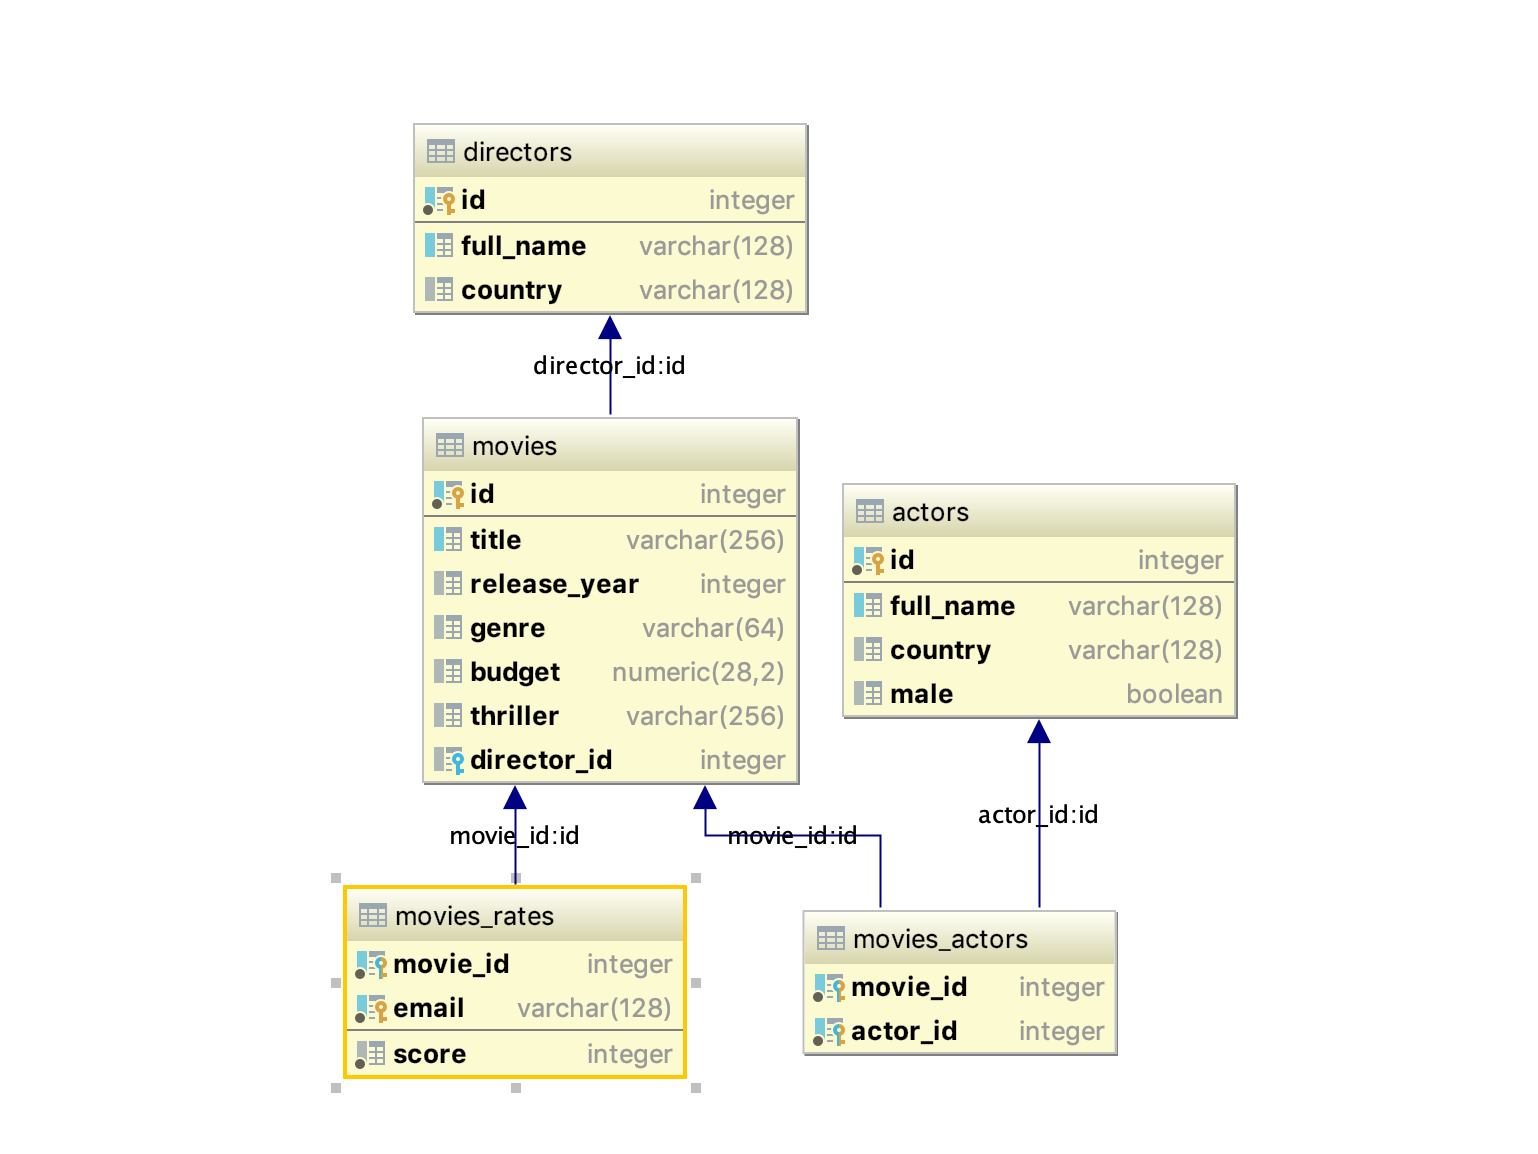
\includegraphics{assets/database-model.png}
\caption{Workshop database model}
\end{figure}

Databases will be populated with below data when postgres container is
launched.

\begin{longtable}[]{@{}rrr@{}}
\caption{directors}\tabularnewline
\toprule
id & full\_name & country\tabularnewline
\midrule
\endfirsthead
\toprule
id & full\_name & country\tabularnewline
\midrule
\endhead
1 & Tim Burton & USA\tabularnewline
2 & James Cameron & Canada\tabularnewline
3 & Steven Spielberg & USA\tabularnewline
4 & Martin Scorsese & UK\tabularnewline
5 & Alfred Hitchcock & USA\tabularnewline
6 & Clint Eastwood & UK\tabularnewline
\bottomrule
\end{longtable}

\begin{longtable}[]{@{}rrrr@{}}
\caption{actors}\tabularnewline
\toprule
id & full\_name & country & male\tabularnewline
\midrule
\endfirsthead
\toprule
id & full\_name & country & male\tabularnewline
\midrule
\endhead
1 & Johnny Depp & USA & true\tabularnewline
2 & Winona Ryder & USA & false\tabularnewline
3 & Russell Crowe & Australia & true\tabularnewline
4 & Joaquin Phoenix & USA & true\tabularnewline
5 & Al Pacino & USA & true\tabularnewline
6 & Robert de Niro & USA & true\tabularnewline
\bottomrule
\end{longtable}

\begin{longtable}[]{@{}rcrrrrr@{}}
\caption{movies}\tabularnewline
\toprule
id & title & release\_year & genre & budget & thriller &
director\_id\tabularnewline
\midrule
\endfirsthead
\toprule
id & title & release\_year & genre & budget & thriller &
director\_id\tabularnewline
\midrule
\endhead
1 & Edward Scissorhands & 1990 & SciFi & 20 &
\url{https://www.yout}\ldots{} & 1\tabularnewline
2 & Gladiator & 2000 & Drama & 103 & \url{https://www.yout}\ldots{} &
7\tabularnewline
\bottomrule
\end{longtable}

\begin{longtable}[]{@{}rr@{}}
\caption{movies\_actors}\tabularnewline
\toprule
movie\_id & actor\_id\tabularnewline
\midrule
\endfirsthead
\toprule
movie\_id & actor\_id\tabularnewline
\midrule
\endhead
1 & 1\tabularnewline
1 & 2\tabularnewline
2 & 3\tabularnewline
2 & 4\tabularnewline
\bottomrule
\end{longtable}

\subsection{API}\label{api}

The below operations are already implemented in our project.

\subsubsection{Queries}\label{queries}

\begin{itemize}
\tightlist
\item
  \textbf{listDirectors:{[}Director!{]}}: It returns the list of
  directors.
\item
  \textbf{listActors:{[}Actor!{]}}:It returns the list of actors.
\item
  \textbf{listMovies:{[}Movie!{]}}: It returns the list of movies.
\item
  \textbf{getMovie(movieId:ID!):Movie}: It returns the movie with given
  id.
\end{itemize}

\subsubsection{Mutations}\label{mutations}

\begin{itemize}
\tightlist
\item
  \textbf{addMovie(request:MovieRequest):Movie!}: It adds a new movie.
\item
  \textbf{addDirector(request:DirectorRequest):Director!}: It adds a new
  director.
\item
  \textbf{deleteDirector(``Identifier of the director''
  direction:ID!):{[}Director!{]}}: It deletes the director with the
  given id.
\end{itemize}

\subsubsection{Subscriptions}\label{subscriptions}

\begin{itemize}
\tightlist
\item
  \textbf{listenDirectorMovies(directorId:ID!):Movie!}: It opens a
  communication with the server and is notified when a new movie is
  created for the passed directorId in the request.
\end{itemize}

\subsection{GraphQL schema}\label{graphql-schema}

The graphql schema for our application looks like this:

\begin{verbatim}
schema {
    # The query root of Workshop GraphQL interface.
    query: Query
    # The root query for implementing GraphQL mutations.
    mutation: Mutation
    # The root query for implementing GraphQL subscriptions.
    subscription: Subscription

}

"""Available queries for Workshop API"""
type Query {
    """It returns the list of directors."""
    listDirectors:[Director!]
    """It returns the list of actors."""
    listActors:[Actor!]
    """It returns the list of movies."""
    listMovies:[Movie!]
    """It returns the movie with the fiven id"""
    getMovie("Movie identifier" movieId:ID!):Movie
}

"""Available mutations for Workshop API"""
type Mutation {
    """I adds a new movie"""
    addMovie(request:MovieRequest):Movie!
    """I adds a new actor"""
    addDirector(request:DirectorRequest):Director!
    """I deletes the director with the fiven identifier"""
    deleteDirector("Identifier of the director" directorId:ID!):[Director!]
}

"""Available subscriptions for Workshop API"""
type Subscription {
    """It returns the movies for a given director"""
    listenDirectorMovies(directorId:ID!):Movie!
}


"""Request info for creating a movie"""
input MovieRequest {
    "Name of the movie"
    title: String!
    "Year when the movie was released"
    year: Int
    "Genre for the movie, supported values should be: SciFi, Drama, Comedy or Action"
    genre: String
    "Budget for the movie, the value is provided in Euro"
    budget: Float!
    "URL in which we can watch the thriller of this movie"
    thriller: String
    "Identifier of director"
    directorId: ID!
}

"""Movie details"""
type Movie {
    "Unique identifier for each movie"
    id: ID!
    "Name of the movie"
    title: String!
    "Year when the movie was released"
    year: Int
    "Genre for the movie, supported values should be: SciFi, Drama, Comedy or Action"
    genre: String
    "Budget for the movie, the value is provided in Euro"
    budget: Float!
    "URL in which we can watch the thriller of this movie"
    thriller: String
    "The director details of the movie"
    director: Director!
    "List of actors for the movie"
    actors("Total of returned actors" total:Int=1): [Actor!]
}

"""Director details"""
type Director{
    "Unique identifier for each director"
    id: ID!
    "Full name of the director"
    fullName: String!
    "Country in which the director was born"
    country: String
}

"""Director creation request"""
input DirectorRequest{
    "Full name of the director"
    fullName: String!
    "Country in which the director was born"
    country: String
}

"""Actor details"""
type Actor {
    "Unique identifier for each actor"
    id: ID!
    "Full name of the actor"
    fullName: String!
    "Country in which the actor was born"
    country: String
    "Gender of actor: Supported values are male or female"
    gender: String
}
\end{verbatim}

\chapter{The GraphQL Playground}\label{the-graphql-playground}

\section{Introduction}\label{introduction}

Once the server is up and ready we can interact with our API by making
use of the \textbf{GraphQL Playground}. There are several desktop
applications that allow us to run our queries against GraphQL API's. On
the other hand, to follow the workshop we will make use of an embedded
web client which is deployed within out api.

Just open
\href{http://localhost:9001/graphql}{ohttp://localhost:9001/graphql} in
your browser.

\begin{figure}
\centering
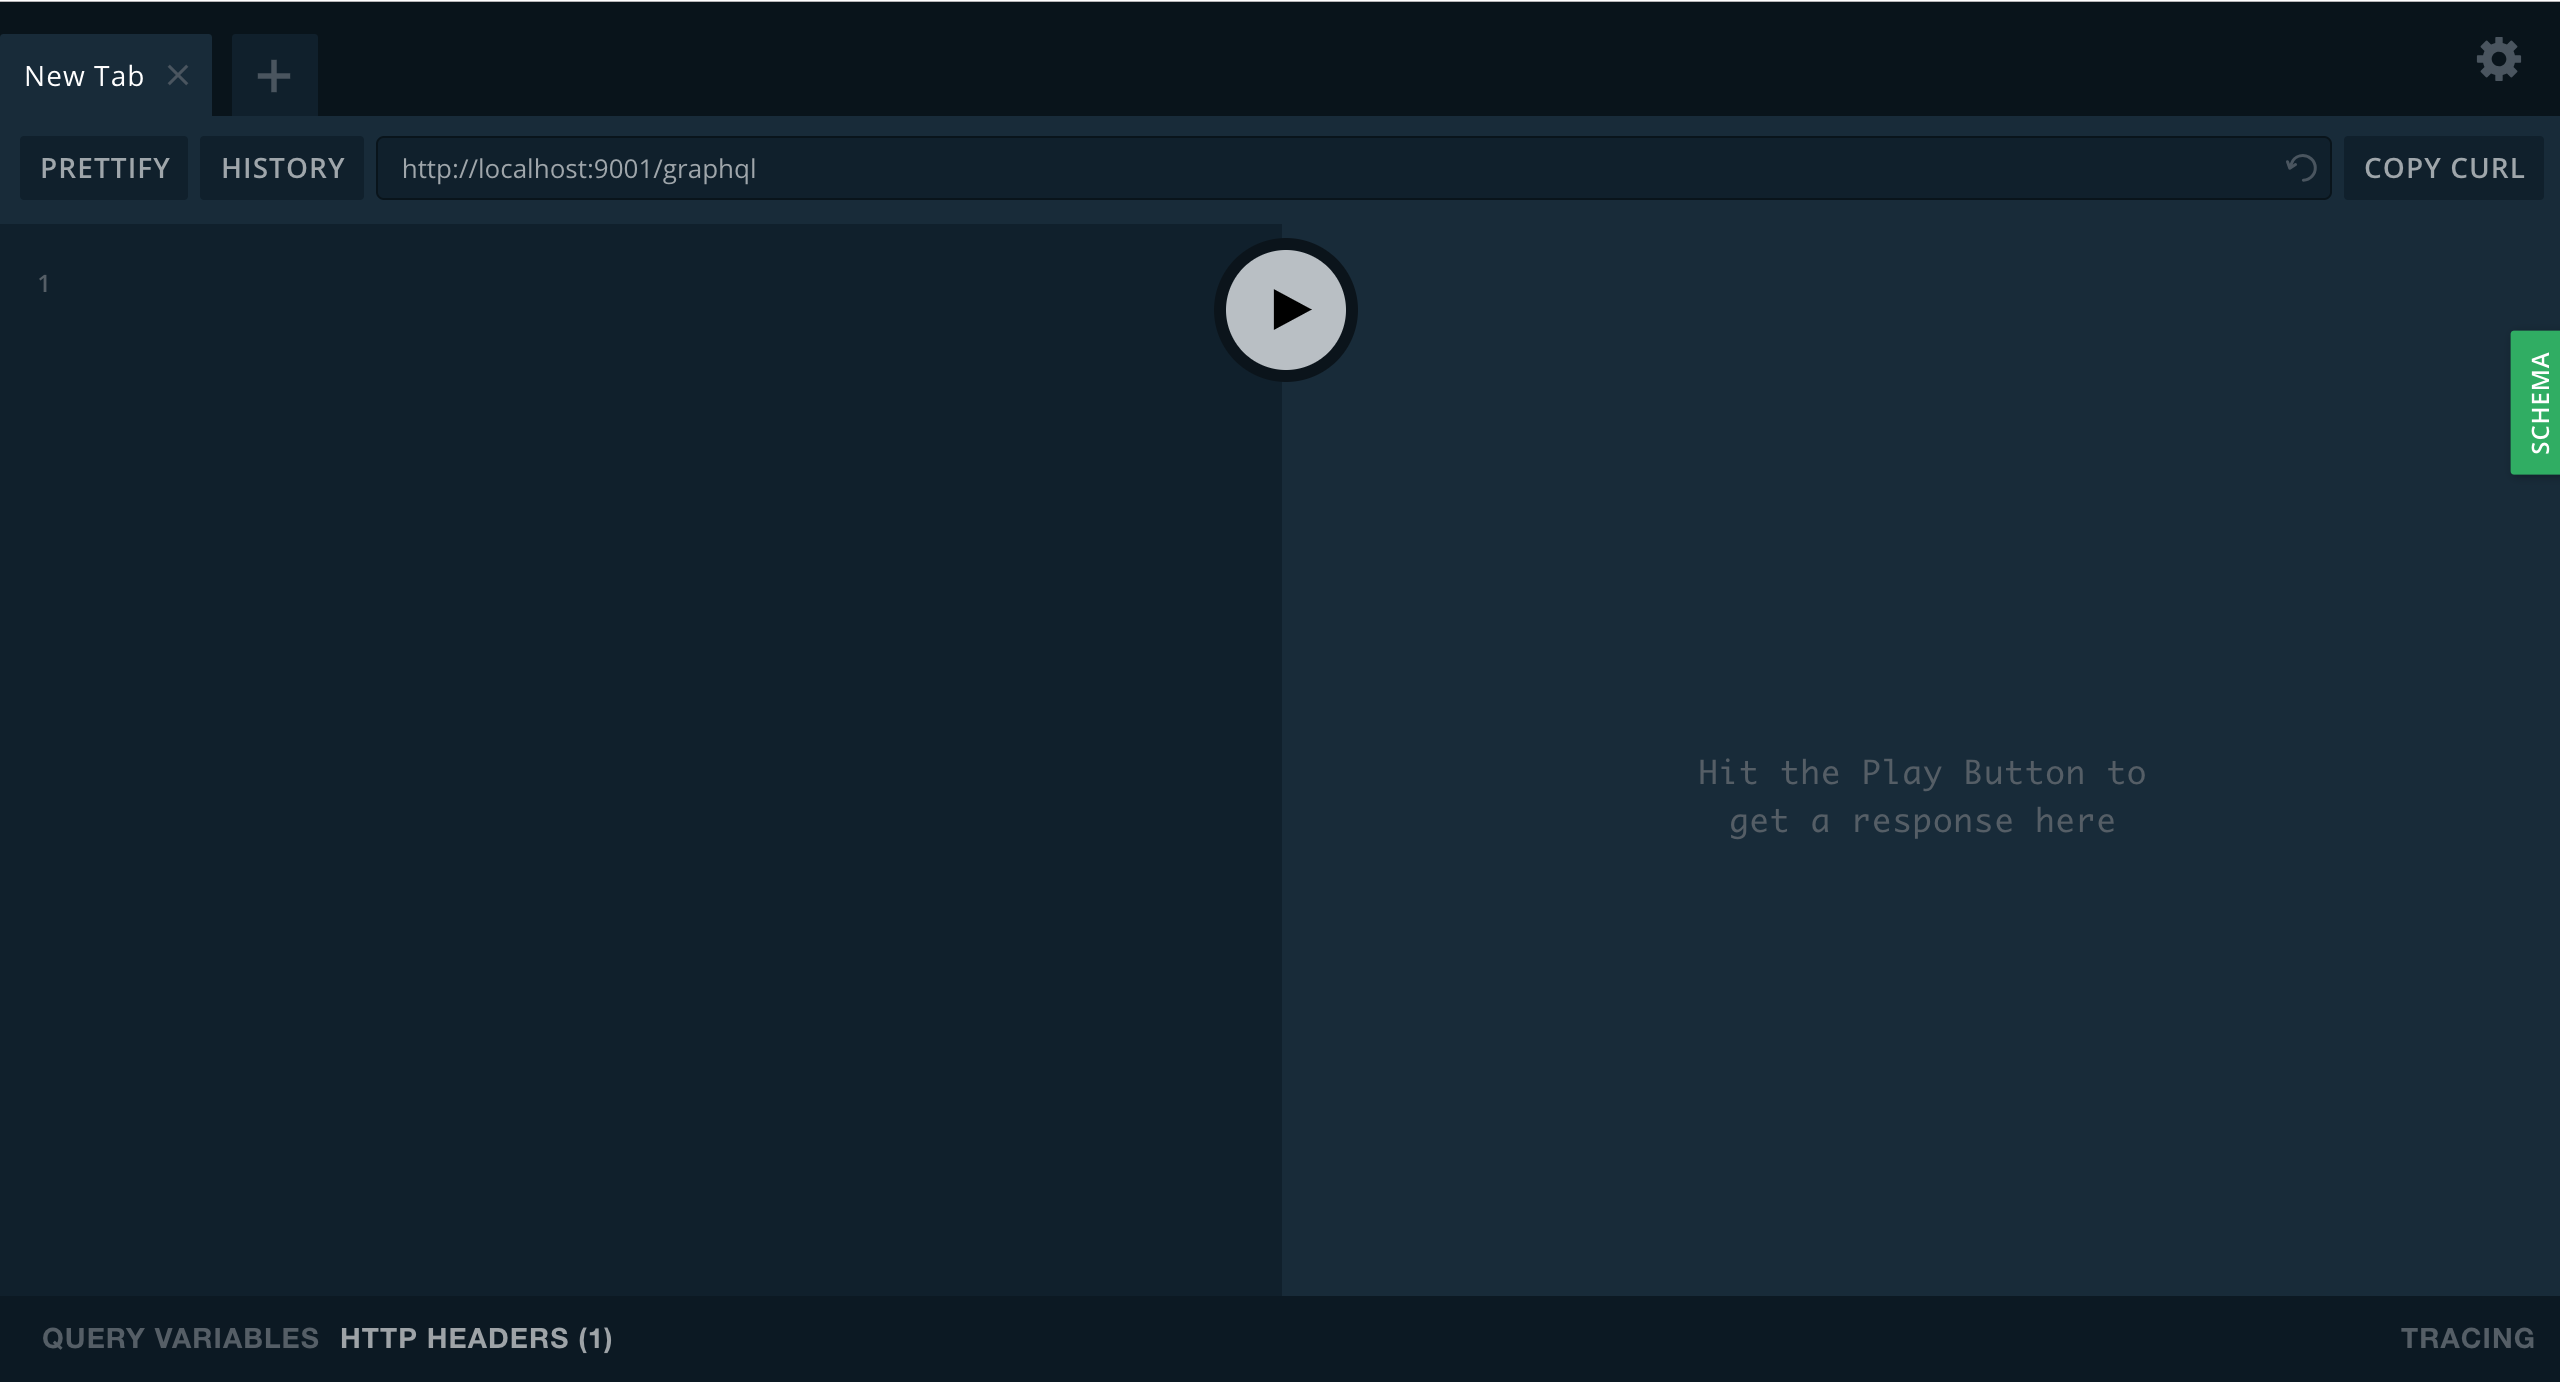
\includegraphics{assets/playground.png}
\caption{GraphQL playground}
\end{figure}

Learn to use ir is not rock science at all. Queries are written on the
left side and the response of these are displayed on the right one.

To check the \textbf{API documentation} we just need to click on the
green button on the right (SCHEMA) and a handy menu will be shown.

\section{GraphQL syntax}\label{graphql-syntax}

GraphQL operations are: queries, mutations and subscriptions. We can run
only one operation per request.

On the other hand we can send more than a query or more than a mutation
at time.

\begin{figure}
\centering
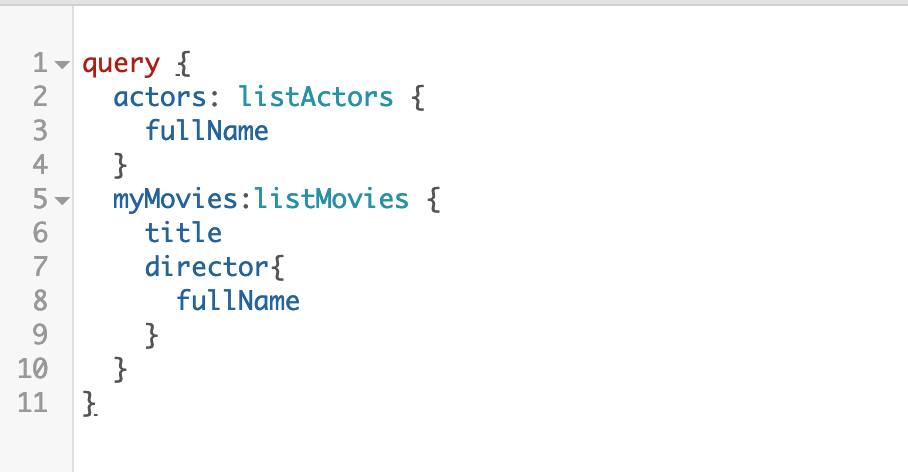
\includegraphics{assets/queries.png}
\caption{Queries with alias}
\end{figure}

\begin{figure}
\centering
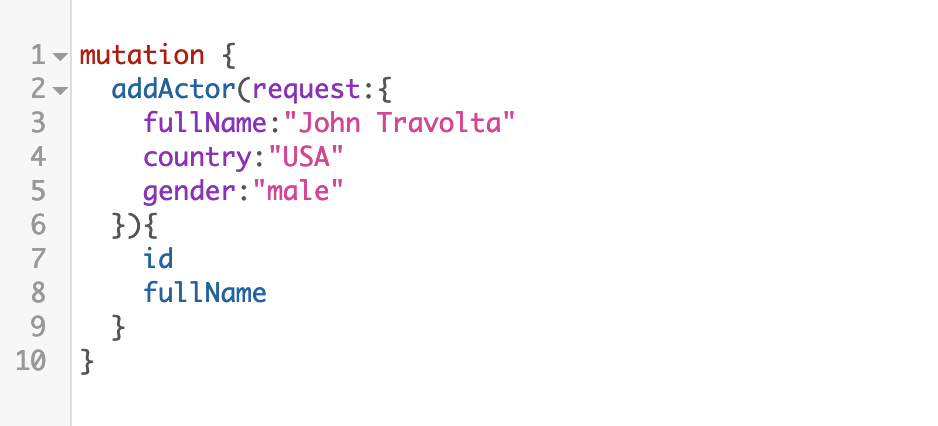
\includegraphics{assets/mutations.png}
\caption{Mutations}
\end{figure}

\begin{figure}
\centering
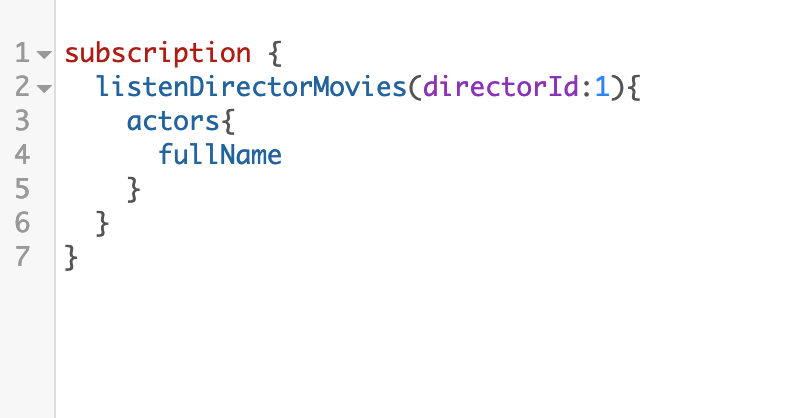
\includegraphics{assets/subscriptions.png}
\caption{Subscriptions}
\end{figure}

\section{Challenges}\label{challenges}

\begin{enumerate}
\def\labelenumi{\arabic{enumi}.}
\tightlist
\item
  Write a query that returns the below details (\textbf{getMovie}) for
  movie with \textbf{id 1}.
\end{enumerate}

\begin{figure}
\centering
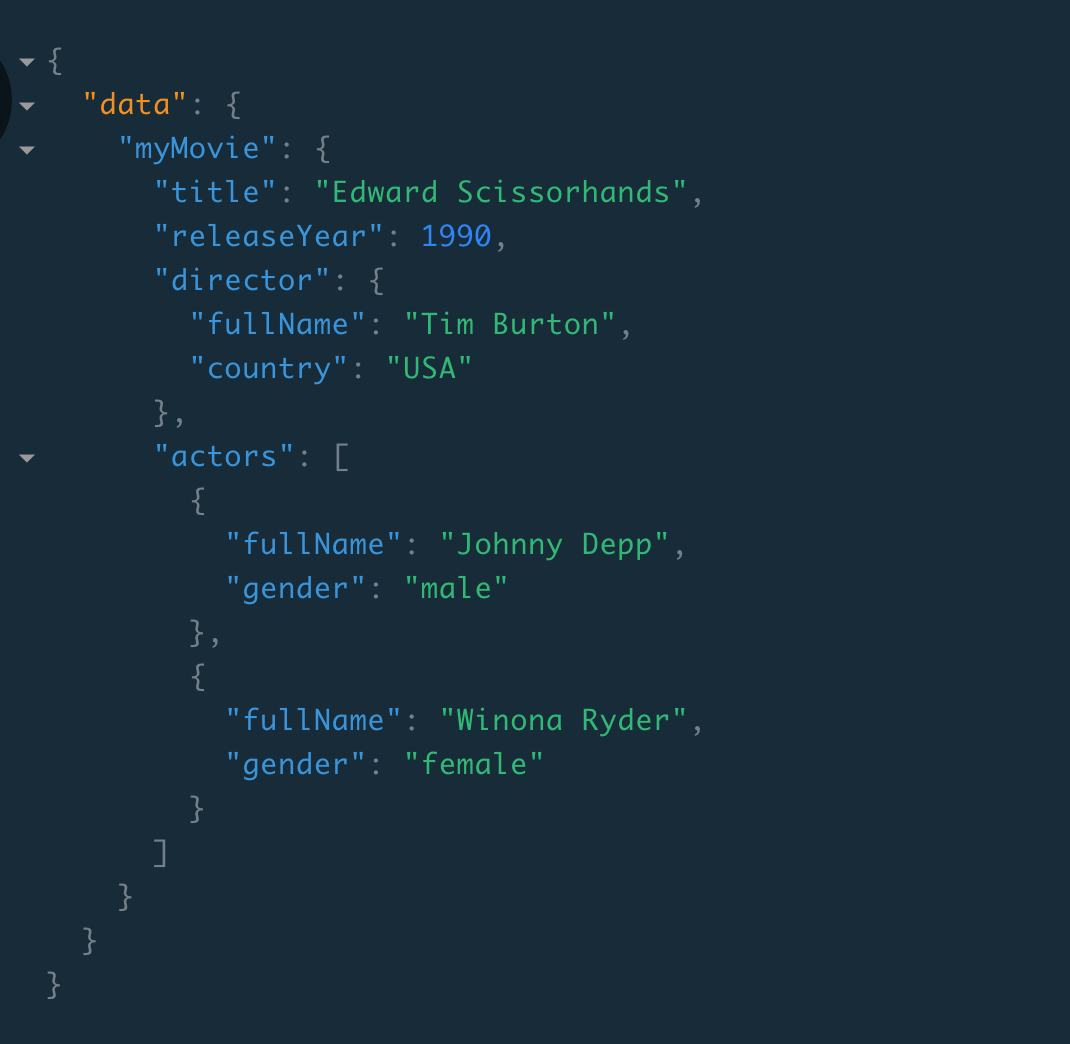
\includegraphics{assets/challenge-one.png}
\caption{Edward Scissorhands}
\end{figure}

\begin{itemize}
\item
  How many actors are returned from the server?
\item
  Are the returned fields the same ones that appear in the picture?
\end{itemize}

\begin{enumerate}
\def\labelenumi{\arabic{enumi}.}
\setcounter{enumi}{1}
\tightlist
\item
  Create a new director (\textbf{addDirector})
\item
  Subscript to the movies for the created director in the previous step.
  (\textbf{listenDirectorMovies})
\item
  Open another tab in your GraphQL Playground and add a new movie in
  which the director is the one that you just created.
  (\textbf{addMovie}).
\item
  Verify that new movie has been notified to the subscription that we
  launched in step 3.
\end{enumerate}

\chapter{GraphQL: Objects}\label{graphql-objects}

\section{Introduction}\label{introduction-1}

The GraphQL specification includes the following default scalar types:
Int, Float, String, Boolean and ID. While this covers most of the use
cases, often you need to support custom atomic data types (e.g.~Date),
or you want a version of an existing type that does some validation. To
enable this, GraphQL allows you to define custom scalar types.
Enumerations are similar to custom scalars, but their values can only be
one of a pre-defined list of strings.

The way to define new scalars or enums in the schema is shown below:

\begin{verbatim}
scalar MyCustomScalar

enum Direction {
  NORTH
  EAST
  SOUTH
  WEST
}

type MyType {
    myAttribute: MyCustomScalar
    direction: Direction
    ...
}
\end{verbatim}

Fields can take arguments as input. These can be used to determine the
return value (eg, filtering search results) or to modify the application
state. These are known as \textbf{field arguments}.

If you have a look at our schema.graphql you can find an example of
usage of a field argument for attribute actors in type Movie.

\section{Code}\label{code}

\subsection{Resolvers}\label{resolvers}

Let's imagine that we have an operation that returns a Employee type and
this type contains an attribute details of type SocialDetails whose
information needs to be taken from an external API. And this attribute
won't be always required by the API consumers. Server should not waste
time on obtaining something that clients do not need.

\textbf{resolvers.js}

\begin{Shaded}
\begin{Highlighting}[]
\ImportTok{export} \ImportTok{default} \OperatorTok{\{}
    \DataTypeTok{Person}\OperatorTok{:} \OperatorTok{\{}
        \DataTypeTok{details}\OperatorTok{:} \AttributeTok{async}\NormalTok{ (}\OperatorTok{\{}\NormalTok{personId}\OperatorTok{\}}\NormalTok{) }\OperatorTok{=>} \OperatorTok{\{}
            \ControlFlowTok{return}\NormalTok{ await }\AttributeTok{getDetailsFromLinkedin}\NormalTok{(personId)}
        \OperatorTok{\},}
    \OperatorTok{\}}
    
\OperatorTok{\}}
\end{Highlighting}
\end{Shaded}

Now, image that SocialDetails can be taken from more than one social
network and we want to permit the consumers to decide which social
network must be used. (It's known as field arguments)

\textbf{schema.graphql.}

\begin{verbatim}
enum Source{
    Linkedin
    Facebook
}
type Person {

  details(source:Source=Linkedin):SocialDetails
}
\end{verbatim}

Our resolver could look like this

\textbf{resolvers.js}

\begin{Shaded}
\begin{Highlighting}[]
\ImportTok{export} \ImportTok{default} \OperatorTok{\{}
    \DataTypeTok{Person}\OperatorTok{:} \OperatorTok{\{}
        \DataTypeTok{details}\OperatorTok{:} \AttributeTok{async}\NormalTok{ (}\OperatorTok{\{}\NormalTok{personId}\OperatorTok{\},\{}\NormalTok{source}\OperatorTok{\}}\NormalTok{) }\OperatorTok{=>} \OperatorTok{\{}
            \ControlFlowTok{if}\NormalTok{ (source }\OperatorTok{===} \StringTok{'Linkedin'}\NormalTok{)}\OperatorTok{\{}
                \ControlFlowTok{return}\NormalTok{ await }\AttributeTok{getDetailsFromLinkedin}\NormalTok{(personId)    }
            \OperatorTok{\}}
            \ControlFlowTok{return}\NormalTok{ await }\AttributeTok{getDetailsFromFacebook}\NormalTok{(personId)}
        \OperatorTok{\},}
    \OperatorTok{\}}
    
\OperatorTok{\}}
\end{Highlighting}
\end{Shaded}

\subsection{Scalars}\label{scalars}

The library \textbf{graphql} provides us with class
\textbf{GraphQLScalarType}. We just need to create a new instance an add
it as a new resolver. An example of scalar type is shown below:

\textbf{scalars.js}

\begin{Shaded}
\begin{Highlighting}[]
\ImportTok{import} \OperatorTok{\{}\NormalTok{GraphQLScalarType}\OperatorTok{\}} \ImportTok{from} \StringTok{'graphql'}\OperatorTok{;}

\KeywordTok{var}\NormalTok{ OddType }\OperatorTok{=} \KeywordTok{new} \AttributeTok{GraphQLScalarType}\NormalTok{(}\OperatorTok{\{}
  \DataTypeTok{name}\OperatorTok{:} \StringTok{'Odd'}\OperatorTok{,}
  \DataTypeTok{serialize}\OperatorTok{:}\NormalTok{ oddValue}\OperatorTok{,}
  \DataTypeTok{parseValue}\OperatorTok{:}\NormalTok{ oddValue}\OperatorTok{,}
  \AttributeTok{parseLiteral}\NormalTok{(ast) }\OperatorTok{\{}
    \ControlFlowTok{if}\NormalTok{ (}\VariableTok{ast}\NormalTok{.}\AttributeTok{kind} \OperatorTok{===} \VariableTok{Kind}\NormalTok{.}\AttributeTok{INT}\NormalTok{) }\OperatorTok{\{}
      \ControlFlowTok{return} \AttributeTok{oddValue}\NormalTok{(}\AttributeTok{parseInt}\NormalTok{(}\VariableTok{ast}\NormalTok{.}\AttributeTok{value}\OperatorTok{,} \DecValTok{10}\NormalTok{))}\OperatorTok{;}
    \OperatorTok{\}}
    \ControlFlowTok{return} \KeywordTok{null}\OperatorTok{;}
  \OperatorTok{\}}
\OperatorTok{\}}\NormalTok{)}\OperatorTok{;}

\KeywordTok{function} \AttributeTok{oddValue}\NormalTok{(value) }\OperatorTok{\{}
  \ControlFlowTok{return}\NormalTok{ value }\OperatorTok{%} \DecValTok{2} \OperatorTok{===} \DecValTok{1} \OperatorTok{?}\NormalTok{ value : }\KeywordTok{null}\OperatorTok{;}
\OperatorTok{\}}
\end{Highlighting}
\end{Shaded}

\textbf{schema.js}

\begin{Shaded}
\begin{Highlighting}[]
\ImportTok{export} \ImportTok{default} \AttributeTok{makeExecutableSchema}\NormalTok{(}\OperatorTok{\{}
    \DataTypeTok{resolvers}\OperatorTok{:} \OperatorTok{\{}
        \DataTypeTok{Odd}\OperatorTok{:}\NormalTok{OddType}
    \OperatorTok{\}}

\OperatorTok{\}}\NormalTok{)}
\end{Highlighting}
\end{Shaded}

You can find more details
\href{https://graphql.org/graphql-js/type/\#graphqlscalartype}{here}

\section{Challenges}\label{challenges-1}

\begin{enumerate}
\def\labelenumi{\arabic{enumi}.}
\tightlist
\item
  Define an enum type Genre whose values are Drama and SciFi (add as
  many other as you want) and use it for attribute genre in type Movie
  and MovieRequest.
\item
  Define an enum Gender and use it for attribute gender in type Actor.
\item
  Define a scalar type Url and use it in attribute thriller of types
  Movie and MovieRequest.
\item
  Define an enum type Currency whose possible values are Euro and
  Dollar. Our API must permit the API consumers to decide in which
  currency they want to obtain attribute budget in type Movie.
\end{enumerate}

\chapter{GraphQL: Operations}\label{graphql-operations}

\section{Introduction}\label{introduction-2}

GraphQL provides us 3 different operations:

\begin{itemize}
\tightlist
\item
  \textbf{Queries}: Operation to retrieve data from the server.
\item
  \textbf{Mutations}: CUD operations: Create, Update and Delete.
\item
  \textbf{Subscriptions}: Create and maintain real time connection to
  the server. This enables the client to get immediate information about
  related events. Basically, a client subscribes to an event in the
  server, and whenever that event ocurrs, the server sends data to the
  client.
\end{itemize}

In our workshop.graphql we will find already implemented operations.

\section{Code}\label{code-1}

Actually there's not difference between implement a query or a mutation.
We will just implament a function that can retrieve 4 arguments:

\begin{itemize}
\tightlist
\item
  \textbf{parent}: The result of the previous resolver call.
\item
  \textbf{args}: The arguments of the resolver's field.
\item
  \textbf{context}: A custom object each resolver can read from/write
  to.
\item
  \textbf{info}: It contains the query AST and more execution
  information.
\end{itemize}

\textbf{queries.js}

\begin{Shaded}
\begin{Highlighting}[]

\ImportTok{export} \KeywordTok{const}\NormalTok{ myQuery }\OperatorTok{=}\NormalTok{ (parentValue}\OperatorTok{,}\NormalTok{ args}\OperatorTok{,}\NormalTok{ ctx}\OperatorTok{,}\NormalTok{info) }\OperatorTok{=>} \OperatorTok{\{}
    \ControlFlowTok{return} \OperatorTok{\{}
        
    \OperatorTok{\}}
\OperatorTok{\};}
\end{Highlighting}
\end{Shaded}

\textbf{mutations.js}

\begin{Shaded}
\begin{Highlighting}[]
\ImportTok{export} \KeywordTok{const}\NormalTok{ myMutation }\OperatorTok{=}\NormalTok{ (parentValue}\OperatorTok{,}\NormalTok{ args}\OperatorTok{,}\NormalTok{ ctx}\OperatorTok{,}\NormalTok{ info) }\OperatorTok{=>} \OperatorTok{\{}
    \ControlFlowTok{return} \OperatorTok{\{}
              
    \OperatorTok{\}}
\OperatorTok{\};}
\end{Highlighting}
\end{Shaded}

Subscriptions looks a little bit different because we need to register
to an event.

\textbf{subscriptions.js}

\begin{Shaded}
\begin{Highlighting}[]
\ImportTok{export} \KeywordTok{const}\NormalTok{ listenChangesInTeam }\OperatorTok{=} \OperatorTok{\{}
    \DataTypeTok{subscribe}\OperatorTok{:}\NormalTok{ (}
\NormalTok{        (_}\OperatorTok{,} \OperatorTok{\{}\NormalTok{teamId}\OperatorTok{\}}\NormalTok{) }\OperatorTok{=>} \OperatorTok{\{}
            \ControlFlowTok{return} \VariableTok{pubsub}\NormalTok{.}\AttributeTok{asyncIterator}\NormalTok{(}\VerbatimStringTok{`teams.}\SpecialCharTok{$\{}\NormalTok{teamId}\SpecialCharTok{\}}\VerbatimStringTok{`}\NormalTok{)}\OperatorTok{;}
        \OperatorTok{\}}
\NormalTok{    )}\OperatorTok{,}
    \DataTypeTok{resolve}\OperatorTok{:}\NormalTok{ (payload}\OperatorTok{,}\NormalTok{ args}\OperatorTok{,}\NormalTok{ context}\OperatorTok{,}\NormalTok{ info) }\OperatorTok{=>} \OperatorTok{\{}
        \ControlFlowTok{return}\NormalTok{ payload}\OperatorTok{;}
    \OperatorTok{\}}
\OperatorTok{\}}
\end{Highlighting}
\end{Shaded}

\section{Challenges}\label{challenges-2}

\begin{enumerate}
\def\labelenumi{\arabic{enumi}.}
\tightlist
\item
  Implement operations \textbf{addActor} and \textbf{deleteActor}.
\item
  Implement operation \textbf{rateMovie} that retrieves a new Input type
  MovieRateRequest. MovieRateRequest contains the movieID, the user
  email and the score. The operation will persist data into table
  \textbf{movies\_rates} and will return the Movie.
\item
  Modify type Movie and add a new attribute rate whose value is the
  average score for all the given rates.
\item
  Modify operation addMovie. Add a new attribute actorsId (array with
  the id's of the actors).
\item
  Define a new query \textbf{getMovieRate} that retrieves an argument
  movieId and the output type is MovieRate. The output must look like
  this:
\end{enumerate}

\begin{Shaded}
\begin{Highlighting}[]
\FunctionTok{\{}
  \DataTypeTok{"rate"}\FunctionTok{:} \StringTok{"7"}\FunctionTok{,}
  \DataTypeTok{"rates"}\FunctionTok{:} \OtherTok{[}
    \FunctionTok{\{}
      \DataTypeTok{"email"}\FunctionTok{:} \StringTok{"john.doe@mail.com"}\FunctionTok{,}
      \DataTypeTok{"score"}\FunctionTok{:} \DecValTok{8}
    \FunctionTok{\}}\OtherTok{,}
    \FunctionTok{\{}
      \DataTypeTok{"email"}\FunctionTok{:} \StringTok{"john.doe@mail.com"}\FunctionTok{,}
      \DataTypeTok{"score"}\FunctionTok{:} \DecValTok{6}
    \FunctionTok{\}}\OtherTok{,}
  \OtherTok{]}
\FunctionTok{\}}
\end{Highlighting}
\end{Shaded}

\begin{enumerate}
\def\labelenumi{\arabic{enumi}.}
\setcounter{enumi}{4}
\tightlist
\item
  Create a new subscription \textbf{listenRates}. This operation
  retrieves an argument movieId and It displays the new rates for the
  given movieId.
\end{enumerate}

\chapter{GraphQL: Interfaces and
Unions}\label{graphql-interfaces-and-unions}

\section{Introduction}\label{introduction-3}

An interface exposes a certain set of fields that a type must include to
implement the interface.

\textbf{schema.graphql}

\begin{verbatim}
interface Restaurant {
    id:ID!
    name: String!
}

type Indian implements Restaurant{
    id:ID!
    name: String!
    brewedBeer:Boolean!
}

type Burger implements Restaurant{
    id:ID!
    name: String!
    vegetarianOptions: Boolean!
}

type Query{
    listRestaurants: [Restaurant!]
}
\end{verbatim}

Unions are identical to interfaces, except that they don't define a
common set of fields. Unions are generally preferred over interfaces
when the possible types do not share a logical hierarchy.

\begin{verbatim}
union Item = Food | Electronic | Customer

type Electronic {
    size: Float
    weight: Float
}

type Food {
    family: String
}

type Customer {
    fullName: String
    zip: String
}
type Query{
    listItems: [Item!]
}
 
\end{verbatim}

\section{Fragments}\label{fragments}

Fragments are powerful technique when we are consuming a query that
returns an Interface or an Union. They are used to define what
attributes we want to obtain from the server depending on the type of
the concrete element.

\begin{verbatim}
query {
    listRestaurants:{
        id
        name
        ... on Indian {
            brewedBeer
        }
        ... on Burger {
            vegetarianOptions
        }
        __typename
    }
}  
\end{verbatim}

\section{Code}\label{code-2}

To implement a new operation with interfaces or unions is easy. We just
need to do it as we did in the previous chapter
\protect\hyperlink{GraphQL:-Operations}{GraphQL: Operations}

On the other hand, we need to define new resolvers to make the server
understand which kind of inherited type it must return. Below we can
find a real example:

\textbf{resolvers.js}

\begin{verbatim}
export default {
    Url: Url,
    Query:{
    
    },
    Mutation: {
    
    },
    Restaurant: {
        __resolveType(restaurant, context, info){
            if(restaurant.brewedBeer){
                return 'Indian';
            }
            return 'Burger'
        },
    }
    ...
}
\end{verbatim}

\section{Challenges}\label{challenges-3}

\begin{itemize}
\tightlist
\item
  Define an interface Person with commons attributes for Actor and
  Director. Add a new query listPeople that returns a list of people
  ({[}Person!{]}).
\item
  Define an union named Item that could be a Movie or an Actor. Add an
  operations listItems that return the full list of Items. {[}Item!{]}
\end{itemize}

\chapter{GraphQL: Directives}\label{graphql-directives}

\section{Introduction}\label{introduction-4}

A GraphQL schema describes directives which are used to annotate various
parts of a GraphQL document as an indicator that they should be
evaluated differently by a validator, executor, or client tool such as a
code generator. GraphQL implementations should provide the \citet{skip}
and \citet{include} directives. GraphQL implementations that support the
type system definition language must provide the \citet{deprecated}
directive if representing deprecated portions of the schema. Directives
must only be used in the locations they are declared to belong in. In
this example, a directive is defined which can be used to annotate a
field:
\href{https://facebook.github.io/graphql/draft/\#sec-Type-System.Directives}{facebook.github.io/graphql}

Authorization is a good and common scenario in which we usually will
make use of directives. We could control what users are allowd to fetch
an object (or even an attribute) from the server.

\begin{verbatim}

directive @isAuthenticated on FIELD | FIELD_DEFINITION
directive @hasRole(role: String) on FIELD | FIELD_DEFINITION

\end{verbatim}

or for clients tools as It was mentioned on the above paragraph.

\begin{verbatim}
directive @deprecated(
  reason: String = "No longer supported"
) on FIELD_DEFINITION | ENUM_VALUE


type ExampleType {
  newField: String
  oldField: String @deprecated(reason: "Use `newField`.")
}
\end{verbatim}

\section{Code}\label{code-3}

From my point of view, this could be the challenging part when
implementinga GraphQL API. Have a look at
\href{https://www.apollographql.com/docs/graphql-tools/schema-directives.html}{apollographql.com}
to understand how we can implement our own directives.

Below a very basic example of directive.

\textbf{directives.js}

\begin{Shaded}
\begin{Highlighting}[]
\ImportTok{import} \OperatorTok{\{}\NormalTok{ SchemaDirectiveVisitor }\OperatorTok{\}} \ImportTok{from} \StringTok{"graphql-tools"}\OperatorTok{;}

\KeywordTok{class}\NormalTok{ DeprecatedDirective }\KeywordTok{extends}\NormalTok{ SchemaDirectiveVisitor }\OperatorTok{\{}
  
  \AttributeTok{visitFieldDefinition}\NormalTok{(field) }\OperatorTok{\{}
    \VariableTok{field}\NormalTok{.}\AttributeTok{isDeprecated} \OperatorTok{=} \KeywordTok{true}\OperatorTok{;}
    \VariableTok{field}\NormalTok{.}\AttributeTok{deprecationReason} \OperatorTok{=} \KeywordTok{this}\NormalTok{.}\VariableTok{args}\NormalTok{.}\AttributeTok{reason}\OperatorTok{;}
  \OperatorTok{\}}

  \AttributeTok{visitEnumValue}\NormalTok{(value) }\OperatorTok{\{}
    \VariableTok{value}\NormalTok{.}\AttributeTok{isDeprecated} \OperatorTok{=} \KeywordTok{true}\OperatorTok{;}
    \VariableTok{value}\NormalTok{.}\AttributeTok{deprecationReason} \OperatorTok{=} \KeywordTok{this}\NormalTok{.}\VariableTok{args}\NormalTok{.}\AttributeTok{reason}\OperatorTok{;}
  \OperatorTok{\}}
\OperatorTok{\}}
\end{Highlighting}
\end{Shaded}

Once we've implemented the directive , we just need to add the
directives as shown below:

\textbf{schema.js}

\begin{Shaded}
\begin{Highlighting}[]
\ImportTok{export} \ImportTok{default} \AttributeTok{makeExecutableSchema}\NormalTok{(}\OperatorTok{\{}
\NormalTok{    typeDefs}\OperatorTok{,}
\NormalTok{    resolvers}\OperatorTok{,}
    \DataTypeTok{schemaDirectives}\OperatorTok{:} \OperatorTok{\{}
        \DataTypeTok{dreprecated}\OperatorTok{:}\NormalTok{ DeprecatedDirective}\OperatorTok{,}
        
    \OperatorTok{\},}
\NormalTok{    ...}
\OperatorTok{\}}\NormalTok{)}\OperatorTok{;}
\end{Highlighting}
\end{Shaded}

\section{Challenges}\label{challenges-4}

\begin{enumerate}
\def\labelenumi{\arabic{enumi}.}
\tightlist
\item
  Create a directive \citet{uppercase} that can be assigned to fields.
  This directive will transform the value of the attribute into
  uppercase. The directive declaration will look lie this
\end{enumerate}

\begin{verbatim}
directive @uppercase on FIELD_DEFINITION
\end{verbatim}

\begin{enumerate}
\def\labelenumi{\arabic{enumi}.}
\setcounter{enumi}{1}
\tightlist
\item
  Create a directive \citet{multiply} with an attribute factor. The
  directive declaration should look like this
\end{enumerate}

\begin{verbatim}
directive @multiply (
    factor: Int!
) on FIELD_DEFINITION
\end{verbatim}

And when the directive is assigned to an field its value will be
multiplied by the given factor.

\begin{verbatim}
input CarRequest {
    km:Int! @multiply(factor:2)
}
\end{verbatim}

\chapter{Challenges Solution}\label{challenges-solution}

This workshop follows a story, and you should not start a new chapter if
you did not complete the purposed challenges in the previous chapters.

The workshop is completely open source and elaborated with great
dedication and effort. So if you are taken the workshop is due to you
want to learn GraphQL. That's why I invite you to try to solve all the
purposed challenges by yourself.

On the other hand, you could be stuck in one of the chapters. Just in
that case, you could checkout the solutions for the challenges.

\begin{enumerate}
\def\labelenumi{\arabic{enumi}.}
\setcounter{enumi}{3}
\tightlist
\item
  GraphQL: Objects - branch: feature/objects
\item
  GraphQL: Operations - branch: feature/operations
\item
  GraphQL: Interfaces and unions - branch: feature/interfaces-unions
\item
  GraphQL: Directives - branch: feature/directives
\end{enumerate}

\begin{quote}
Please if you have any doubt contact me at
\href{mailto:ivan.corrales.solera@gmail.com}{\nolinkurl{ivan.corrales.solera@gmail.com}}
\end{quote}

\begin{itemize}
\tightlist
\item
  \href{https://www.apollographql.com/docs/}{Apollo GraphQL}
\item
  \href{https://facebook.github.io/graphql/}{GraphQL Specification}
\end{itemize}


\end{document}
